% !TEX TS-program = LuaLaTeX
% !TEX encoding = UTF-8 Unicode
%%%%%%%%%%%%%%%%%%%%%%%%%%%%%%%%%%%%%%%%%%%%%%%%%%%%%%%%%%%%%%%%%%%%%%%%%%%%%%%%%%%%%%%%%%
%% Option for language settings and equations adjusment,
%% http://www.tug.org/texlive/Contents/live/texmf-dist/doc/fonts/bera/bera.txt
\documentclass[swedish, english, 11pt ]{article}
\usepackage{babel}
\usepackage[T1]{fontenc}
% Makes utf8 in pdf mode
\usepackage[utf8]{luainputenc}

%%%%%%%%%%%%%%%%%%%%%%%%%%%%%%%%%%%%%%%%%%%%%%%%%%%%%%%%%%%%%%%%%%%%%%%%%%%%%%%%%%%%%%%%%%
\usepackage{stackrel}
\usepackage[leqno]{amsmath}
\usepackage{lualatex-math}
\usepackage{amssymb}
\usepackage{rotating}
\usepackage{array}
\usepackage{lastpage}
\usepackage{multirow}
\usepackage{arydshln}
\usepackage{longtable}
\usepackage{dcolumn}
\usepackage{enumitem}
\setlist[enumerate]{ topsep=1em,itemsep=0.8em, itemindent=0.5em, 
  labelsep=0.7em, labelindent=\parindent, leftmargin=* }
% For boxes and other stuff inside align and equations
% begin{empheq}[ box = \fbox]{align*} ... \end{empheq}                                                
\usepackage{empheq} 
\newcommand*\textfbox[2][Title]{%
  \begin{tabular}[b]{@{}c@{}}#1\\\fbox{#2}\end{tabular}}
  
%%%%%%%%%%%%%%%%%%%%%%%%%%%%%%%%%%%%%%%%%%%%%%%%%%%%%%%%%%%%%%%%%%%%%%%%%%%%%%%%
\addto\captionsenglish{\renewcommand{\figurename}{Figur}}
\addto\captionsenglish{\renewcommand{\contentsname}{Innehållsförteckning}}
\addto\captionsenglish{\renewcommand{\tablename}{Tabell}}
\addto\captionsenglish{\renewcommand{\listfigurename}{Figurförteckning}}
\addto\captionsenglish{\renewcommand{\listtablename}{Tabellförteckning}}
%% Change name of bibliograph, when cite{} is used
\addto\captionsenglish{\renewcommand{\bibname}{Referenser}}

\usepackage{booktabs}
%%%%%%%%%%%%%%%%%%%%%%%%%%%%%%%%%%%%%%%%%%%%%%%%%%%%%%%%%%%%%%%%%%%%%%%%%%%%%%%%%%%%%%%%%%
%%footmisc controls the footnotes
\usepackage[bottom, flushmargin, hang, multiple]{footmisc}
\setlength{\footnotemargin}{3.5mm}
\usepackage{eurosym}


\usepackage{pdflscape}
%% \begin{landscape}...\end{landscape}

%%%%%%%%%%%%%%%%%%%%%%%%%%%%%%%%%%%%%%%%%%%%%%%%%%%%%%%%%%%%%%%%%%%%%%%%%%%%%%%%%%%%%%%%%%
%% Macros used in the paper, the [2] means number of arguments used in
%% the macro. Amsthm is package for Theorem
\usepackage{acronym}

%%\renewcommand{\setthesubsection}{\arabic{subsection}}
\newcommand{\email}[1]{{\normalfont\texttt{#1}}}
\newcommand{\code}[1]{\mbox{\texttt{#1}}}
\newcommand{\pkg}[1]{{\normalfont\fontseries{b}\selectfont #1}}
\newcommand{\proglang}[1]{\textsf{#1}}
\newcommand{\sign}[1]{\ensuremath{\text{\textsf{#1}}}}
\newcommand{\HRule}[1]{\rule{#1}{0.5mm}}
\newcommand{\R}{\proglang{R}\, }
\newcommand{\D}{\pkg{data.table()}\,}
\newcommand{\CC}[1]{\code{#1()}\,}
\newcommand{\tb}[1]{\textbf{#1}}
\newcommand{\un}[1]{\textsc{#1}}
\newcommand{\unn}[1]{\underline{\textit{\scalebox{1.4}{#1}}}}
\newcommand{\fullref}[1]{\ref{#1} (se sida~\pageref{#1})}
%% These codes are used in this document a lot
\newcommand{\inputy}[1]{\input{#1}\unskip}
% For variables, $\var{1}{2}$
\newcommand{\var}[2]{\ensuremath{\textbf{#1}_{#2} }}
\newcommand{\vars}[2]{\ensuremath{\textsf{#1}_{\textrm{#2}}}}
\usepackage{verbatim}
\newcommand\codeHighlight[1]{\textcolor[rgb]{1,0,0}{\textbf{#1}}}
\newcommand{\textRM}[1]{\textrm{{\scriptsize #1}}}

% Command för index
\DeclareRobustCommand{\EX}[2][{\sign{E}}]{\ensuremath{#1}\left[{#2}\right]}
\DeclareRobustCommand{\EV}[2][{\sign{V}}]{\ensuremath{#1}\left[{#2}\right]}
\DeclareRobustCommand{\EM}[2][{\sign{M}}]{\ensuremath{#1}\left[{#2}\right]}
\DeclareRobustCommand{\IF}[2][{\sign{IF}}]{\ensuremath{#1}\left[{#2}\right]}
%%%%%%%%%%%%%%%%%%%%%%%%%%%%%%%%%%%%%%%%%%%%%%%%%%%%%%%%%%%%%%%%%%%%%%%%%%%%%%%%%%%%%%%%%%
%% Control over caption and subfig

%% Options for fancy heading, section layout
 % Layout options
\usepackage{etoolbox} %ifstrequal etc
\usepackage{tikz}
\usetikzlibrary{shapes,shadows,calc}
\pgfdeclareimage[width = 0.1\paperwidth]{kriita}{Logo/paylevo.png}
%% 1125/1400*0.95
\IfFileExists{Logo/paylevo.png}
{
\pgfdeclareimage[width = 0.95\paperwidth]{core}{Logo/paylevo.png}
} {
\pgfdeclareimage[width = 0.6\paperwidth]{core}{../Logo/paylevo1.png}
}
\newcommand\SecTitle[4]{% can use \hspace*{-1.5}

\begin{tikzpicture}
  \node[inner xsep=0pt,minimum height=3cm,text width=1\textwidth,
      align=left,left color=gray,  right color=white, signal to=#1,font=\Huge,anchor=#2] 
          at (#3,0) {\hspace*{0.25\textwidth}\textsf{#4}};
\end{tikzpicture}%
}


\newcommand\SecTitleSub[4]{%
\begin{tikzpicture}
  \node[inner xsep=0pt,minimum height=1.5cm,text width=0.95\textwidth,
      align=left,left color=gray, right color=white, signal to=#1,font=\huge,anchor=#2] 
          at (#3,0) {\hspace*{0.15\textwidth}\textsf{#4}};
\end{tikzpicture}%
}

\usepackage[textfont=small, labelfont=bf, format=plain,%
	position=top, justification=raggedright,width=.9\textwidth]{caption}
\usepackage[font=footnotesize, labelfont=bf]{subfig}

\usepackage{xcolor}
%\definecolor{gray1}{gray}{0.2}
\definecolor{darkred}{rgb}{0.545,0,0}
\definecolor{midnightblue}{rgb}{0.098,0.098,0.439}
\definecolor{darkred}{rgb}{0.176,0.23,0.31}
\definecolor{indianred}{rgb}{0.545,0,0} % Between 0 and 1
\definecolor{crimson}{RGB}{220,20,60} 
\definecolor{gray1}{RGB}{3,3,3}
%% Make color in equations
\makeatletter
\let\reftagform@=\tagform@
\def\tagform@#1{\maketag@@@{(\ignorespaces\textcolor{blue}{#1}\unskip\@@italiccorr)}}
\renewcommand{\eqref}[1]{\textup{\reftagform@{\ref{#1}}}}
\makeatother
\usepackage{hyperref}
\hypersetup{%
  breaklinks = {true},
  colorlinks= {true},
  linkcolor={indianred},
  citecolor={indianred},
  urlcolor = {midnightblue},
  unicode  = {true},
  bookmarksnumbered = {true},
  bookmarksopen = {true}
 }



%%%%%%%%%%%%%%%%%%%%%%%%%%%%%%%%%%%%%%%%%%%%%%%%%%%%%%%%%%%%%%%%%%%%%%%%%%%%%%%%%%%%%%%%%%
%% Options for fancy heading and alike
\usepackage{fancyhdr}
\pagestyle{fancy}
\oddsidemargin = 12pt
\textwidth = 450pt
\headsep = 40pt
\voffset = -10pt
\fancyheadoffset{30pt}
\headheight = 21pt
\textheight = 620pt
\pagenumbering{arabic}
\renewcommand{\headrulewidth}{0.5pt}
\setlength{\footskip}{0in}

\fancyhf{}
\fancyhead[C]{\textit{ \thepage\--(\pageref{LastPage}) }}
\fancyhead[L]{\pgfuseimage{kriita}}
\fancyhead[R]{\footnotesize \textsc{Analys}}
\renewcommand\headrule
{{\color{midnightblue}%
  \hrule height 1pt
         width\headwidth
  \vspace{1pt}%
  \hrule height 0.4pt
         width\headwidth
  \vspace{-4pt}
  }}
  

%%
%%
%%%%%%%%%%%%%%%%%%%%%%%%%%%%%%%%%%%%%%%%%%%%%%%%%%%%%%%%%%%%%%%%%%%%%%%%%%%%%%%%%%%%%%%%%%
%% Control over (indrag) and equation, respectively
\setlength{\parindent}{0.7cm}
\numberwithin{equation}{section}
% Dir to search for graphs
\graphicspath{{graf/}{graf_manual/}{all/}{FAST_GRAF/}}
\DeclareGraphicsExtensions{.pdf}

\usepackage{Sweave}
%\SweaveOpts{ echo = TRUE, keep.source = TRUE}

%% Lisiting options
\usepackage{listings}
\DeclareCaptionFont{white}{\color{white}}
\DeclareCaptionFormat{listing}{\colorbox[cmyk]{0.43, 0.35, 0.35,0.01}{\parbox{0.95\textwidth}{\hspace{10pt}#1#2#3}}}
\captionsetup[lstlisting]{format=listing,labelfont=white,textfont=white, singlelinecheck=false, margin=0pt, font={bf,footnotesize}}
\definecolor{light-gray}{gray}{0.95}
\lstset{	language=R,
		keywordstyle=\color{blue},
		numbers=right, 
                	numberstyle=\tiny, 
                alsoletter={.},
                breaklines=true,
                backgroundcolor=\color{light-gray},
                xleftmargin=5mm,
                xrightmargin=8mm,
                numbersep=5pt,
                 frame=shadowbox,
                 showstringspaces=false
                } 



\usepackage{fontspec}
\usepackage{fontspec}
\setmainfont[Ligatures=TeX]{Latin Modern Roman}
\setsansfont{Latin Modern Sans}
\linespread{1.3}% Mellanrum i texter
\frenchspacing % remove extra space after punctuation
\usepackage[explicit]{titlesec}
%filcenter puts the section heading at middle and adjust with 1em accodingly
% filright, filleft
% titleformat{<label>}[format]{<section apperance>}{<number>}{space}{}{}
\titleformat{\section}
{\normalfont}{}{0em}
{\SecTitle{east}{west}{0\paperwidth}{#1}}


\titleformat{\subsection}
{\normalfont}{}{0em}
{\SecTitleSub{east}{west}{0\paperwidth}{#1}}

\usepackage{Commands}	%\begin{mybox}{<title>} \begin{MyBlock}[<width>]{<title>}



\begin{document}
%%%%%%%%%%%%%%%%%%%%%%%%%%%%%%%%%%%%%%%%%%%%%%%%%%%%%%%%%%%%%%%%%% %%%%%%%%%
\section{Definition} 
\label{sec:1} 
Paylevos verksamhet utgörs av online fakturering, där tanken är att överföra den risk som sker när köpet och 
betalning inte sker på samma gång. Således så kommer Paylevo att "köpa" fakturan och överföra likvida 
medel till företagaren.  Nu så är verksamheten mera komplex, risken är ofta på handlarens sida, men för att 
lösa denna uppgift så kommer vi att låtsas att Paylevo tar risken och på så vis äger varje faktura som skapas 
i systemet.  

Alla fakturor är omvandla till svenska kronor. Följande villkor och statistik gäller initialt:

\begin{enumerate}[label=\emph{\arabic*})]
	\item \textit{Tidsperiod}:  Start (2014-10-01) till  (2016-12-24), vilket gör 
		att en faktura idag är ansedd som en kredit förlust, cirka 4 månader.
	\item \textit{Utgivna fakturor}: Avser även fakturor som slut kunden  ångrat sitt köp, totala antalet är 243 644 st.
	\item \textit{Antal unika kunder}:  74 516 st. %% change
	\item \textit{Inflöde av pengar}:  100 031 141 SEK, är beräknad genom inflöde av likvida medel minus utflödet av pengar. %% change
		Sker på grund av att vi ibland måste returnera pengar till slutkunden. 
	\item \textit{Charges}: Är summan av alla intäkter från inkasso, ränta betalningspåminnelse, transaktionsavgift och fakturaavgift, vilket blir 17 112 513  SEK. %%change
	\item \textit{Förväntad förlust}: Är alla fakturor som idag är ansedda som en kredit förlust och avser endast själva kapital beloppet,  15 139 692  SEK. %%change
	\item \textit{Lönsam kund}: Detta sker på kundnivå, och genom förenkling så bortses här från den kostnad som är förknippad när Paylevo utfärdar en faktura. Men principen för en 
		lönsam kund är \textit{Charges} $-$ \textit{Förväntad förlust}.
\end{enumerate}

Efter att rensat för de kunder där vi har kredit data samt endast för svenska så ser bilden ut enligt följande:

\begin{enumerate}[label=\emph{\arabic*})]
	\item \textit{Utgivna fakturor}: 145 885 st.
	\item \textit{Antal unika kunder}:  52 223 st.
	\item \textit{Inflöde av pengar}:  68 719 278 SEK. 
	\item \textit{Charges}:  13 769 029  SEK.
	\item \textit{Förväntad förlust}:  12 339 323  SEK.
	\item \textit{Procentuella förlust}: Baserad på antal fakturor,  18.8  procent,  och total summa
		18 procent. Dessa siffror är väldigt höga, och stämmer inte. Men för att avgöra de bra från de dåliga så 
		låtsas Paylevo ta risken för alla fakturor.
\end{enumerate}


\begin{equation*}
\label{eq:1}
\textsf{ Customer profitably }=\left\{
\begin{array}{c l}     
    1 & \textrm{  Yes }  \\
    0 & \textrm{No  }  \\
    \end{array}\right.
\end{equation*}


\clearpage
%%%%%%%%%%%%%%%%%%%%%%%%%%%%%%%%%%%%%%%%%%%%%%%%%%%%%%%%%%%%%%%%%% %%%%%%%%%
\section{Data städning} 
\label{sec:2} 
Första steget i analysen är att ta bort data som "stör" modelleringen. Först ut är att ta bort alla variablar som innehar "NA" 
inom sig. Vårt dataset är relativt stort och behöver således inte betyda så mycket om ett par hundra försvinner. I detta 
fall så var det ca 90 st observationer som försvann. Även de variabler som innehar en stor andel NA tas bort, tex 
\textit{DEBTRELIEF\_DATE}. Ytterligare arbete är att sammanställa vissa variablar för att minska variationen. 

\begin{empheq}[box={\textfbox[Minska variation på följande]}]{align*}
	\textRM{DEBT\_NUMBER} 	= & \text{IF } x <  5 \text{ "Låg"} \text{ ELSE } \text{ "Hög"}  \\  
	\textRM{AGE} 	= & \text{IF} x <  30 \text{ "Young"} \text{ ELSE IF }  x >= 30 \& x < 50\text{ "Middle"} \text{ ELSE Old}   \\  
\end{empheq}

Samtidigt så måste även variablar som inte har någon som helst variation inom sig också tas bort\footnote{
	Använder funktionen \code{nearZeroVar()} som tittar på antalet unika värden i relation till stickprovet.

}, tex 
\textit{INCOME\_BUSINESS} och 3 liknande variablar försvinner. Outliers drabbar olika för olika 
modeller, tex beslutträd är inte känslig för outliers medans regressons modeller är det.
Slutligen så avslutas "städningen" genom att dela i analys data i två delar, ena är där modellerna 
skall tränas och andra är test datasetet där prognosen skall utvärderas på. Skulle vi inte göra på detta sätt
så skulle det uppstå en bias eftersom vi utför en prognos på samma dataset som modelleringen utformats inom i.

Först ut är att granska den interna korrelationen för de numeriska variablerna.
Ett stort problem i all modellering arbete är att jobba med väldigt högt korrelerat data i de explanativa variabler\footnote{
	Dvs de variablar som ska användas för att utföra prognosen. 
}.  Orsaken till detta är den interna korrelationen är alldeles för hög och på så viss svårigheter att avgöra vad som korrelerar med 
$y$ - variabeln. 

Följande analys i figur~\ref{fig:correlation} sker endast för de numeriska variablerna. 
Det man kan se är att det finns en väldigt stark korrelation sinsemellan alla x-variabler (översta grafen).
Tex \textit{INCOME} med \textit{INCOME2}, dvs har man haft en hög inkomst föregående år så har man 
även det kommande år.  Således kommer dessa att tas bort. De som tas bort efter att använt en "cutoff" på 
90\% procent är tex \textit{TEXEBLE\_INCOME} och  \textit{FINAL\_TAX} samt ytterligare två till.

 

%%%%%%%%%%%%%%%%%%%%%%%%%%%%%%%%%%%%%%%%%%%%%%%%%%%%%%%%%%%%%%%%%% %%%%%%%%%
\section{Beslutsträd}  
%%%%%%%%%%%%%%%%%%%%%%%%%%%%%%%%%%%%%%%%%%%%%%%%%%%%%%%%%%%%%%%%%% %%%%%%%%%

 Inför arbetet med att hitta den optimala modellen så kommer först att utröna vilka variabler som är 
 viktiga för att utföra en prognos att genomföras.  Just nu är det variable enligt ekvation~\eqref{eq:1}
 som utforskas.
 
Vad som sker enligt nedanstående kodning är att tränings datasetet  splittas i ytterligare 10 delar
och där ett beslutträd skapas i varje, detta utförs 3 gånger. Vi använder ROC för att att hitta 
det bästa trädet. 
\begin{lstlisting}[caption = \textsf{Metod}, language=R]
fitControl <- trainControl(## 10-fold CV
   method = "repeatedcv",
      number = 10,
      summaryFunction = twoClassSummary,
	classProbs = TRUE,
      ## repeated 3 times
          epeats = 3)


 bmFit1 <- train(y = yVar$Profitably,
				x =  xVar,
                	 method = "rpart", 
                	 metric = 'ROC',
                 	trControl = fitControl,
                 	tuneLength = 20)
\end{lstlisting} 




Så baserat på fig~\eqref{fig:imp} så kommer ytterligare variabler att reducerats inför den första 
testomgången och en baseline modell. I princip så väljs de variablar som modellen anser som 
viktigast, skär vid 20. Den variabel som är allra viktigast i beräkna vilken kund som är ansedd som 
vinstgivande är alltså \textit{DEBT\_SUM} följt av SCORING.

Jag kommer att använda Gini måttet i och reducerat trädet med hjälp av komplexitets parametern.
Figur~\eqref{fig:tree1} i sida~\pageref{fig:tree1} fås då. Valet av komplexitet parametern fås genom 
"1SE" regeln, vilket kollar på kolumn "xerror" och "xstd" \footnote{ Cross validation error  och dess standard fel } 

Modellen är en aningen för komplex för att erhålla alla regler. Men kollar vi de regler som fångar upp 
den stora massan ser det ut enligt följande.



\begin{align}
	\text{DEBT\_SUM >= 226 \& DEBT\_NUMBER == 'High' } 	= & \text{Regel 1}  \\  \notag
	\text{[DEBT\_SUM < 226   } 							= &\text{Regel 2} \\   \notag
	\text{DEBT\_SUM >= 226 \& DEBT\_NUMBER != 'High' \& TOTAL\_INCOME < 88000 } = & \text{Regel 3} \notag
\end{align}

\begin{table}[ht]
\centering
\caption{ Summering av modell enligt fig~\eqref{fig:tree1}}
\setlength{\extrarowheight}{2pt}
\begin{tabular}{l>{\sffamily}l c c}
\toprule 
Logisk regel  &  Kreditförlust (utgift) & Vinst (Charges)  & Kreditförlust (\%)   \\
\cmidrule(l){2-4}
	1) & -6 882 924  & 335 216 & 84.96 \\
	 2) & -2 357 855  & 12 173 447  & 5.15  \\
	3)  & -809 985  & 50 608 & 82.49   \\
\bottomrule
\end{tabular}
\label{Q:1}
\end{table}

Så vad säger tabell~\ref{Q:1}, en positiv kreditförlust innebär att man sparat pengar genom att tillämpa 
respektive regel, och en negativ kreditförlust att det är pengarna som företaget sparat.

Skulle vi exempelvis tillämpa regel 1, så skulle vi bespara företaget en kreditförlust på -6 882 924 SEK
(eftersom vi då köpt fakturor för den summa), men eftersom vi tillämpar regeln så kommer vi att förlora en förväntad intäkt\footnote{
	Alla är ju inte dåliga kunder, ca  15.04 äv kunderna är ansedda som bra.
},  335 216   SEK. På samma viss är det för regel två, där vi köper fakturor från folk som har 
en mindre skuld än 226 SEK. På så viss har vi en kreditförlust på -2 357 855 men en 
intäkt på 12 173 447 SEK.

Så för att göra en prognos baserad på nedanstående modell måste vi först hitta den optimala cutoffen. Detta
görs bäst med hjälp av ROC analysen. Först skapas en vektor av sannolikheten baserad på modellen och 
test data.

\begin{table}[ht]
\centering
\caption{ Prognos av modell enligt fig~\eqref{fig:tree1} på test data antal 8152 }
\setlength{\extrarowheight}{2pt}
\begin{tabular}{l>{\sffamily}l c }
\toprule 
Prognos/Utfall &  False & True    \\
\cmidrule(l){2-3}
	False & 947  & 234 \\
	 True & 374  & 6597   \\
	 Accuracy & 0.925 & -- \\
	 Sensitivity & 	 0.966 & -- \\
	  Specificity & 	 0.717 & -- \\
	  Precision (PPV)& 	 0.946 & -- \\
	  Neg predictive value (NPV)& 	 0.802 & -- \\
	  AUC	& 0.872 & --\\
\bottomrule
\end{tabular}
\label{Q:roc}
\end{table}

\begin{align} 
	\text{Accuarcy} =& \frac{\text{TP} + \text{TN}}{\text{P} + \text{N}} \\
	\text{Specificity} =& \frac{\text{TN}}{ \text{TN} + \text{FP}} \\
	\text{Sensitivity} =& \frac{\text{TP}}{ \text{TP} + \text{FN}}  \\
	\text{PPV} =& \frac{\text{TP}}{ \text{TP} + \text{FP}}  \\
	\text{NPV} =& \frac{\text{TN}}{ \text{TN} + \text{FN}}  
\end{align}


\begin{figure}[ht]
\centering
\caption{ROC}
\subfloat[]{
\fbox{	
	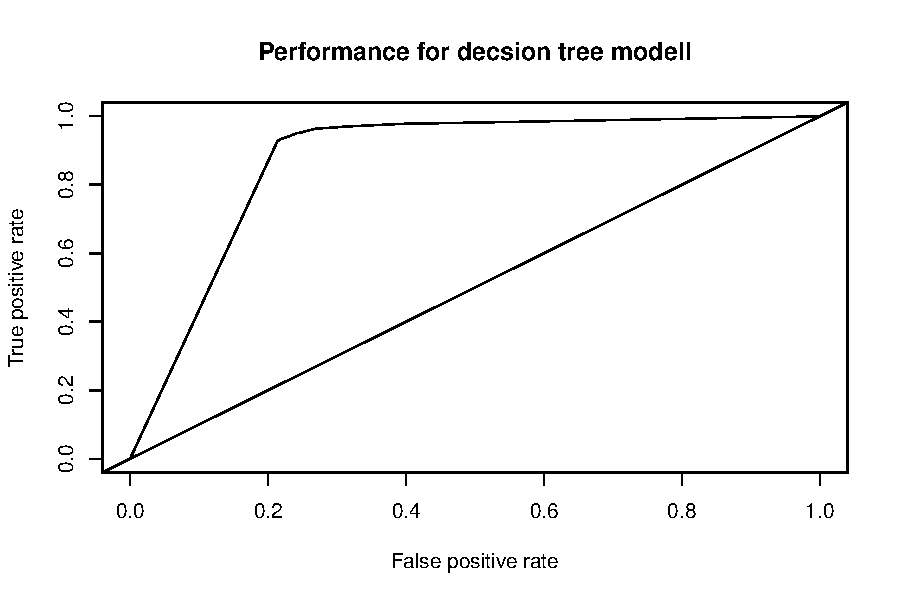
\includegraphics[width=0.45\textwidth,keepaspectratio]{ROCtree}
	}
}
\hfill
\subfloat[]{
\fbox{	
	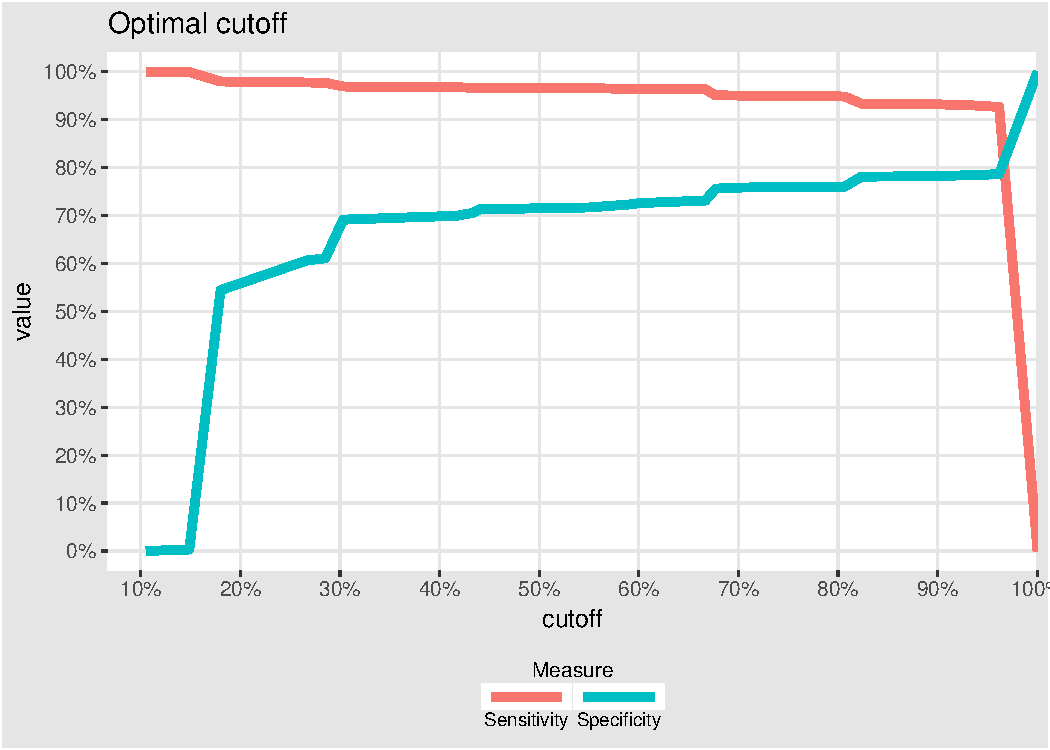
\includegraphics[width=0.45\textwidth,keepaspectratio]{rocOpt}
	}
}	
\label{fig:roc}
\end{figure}





\clearpage

\section{Bagging \& boosting}
The best way to evaluate and train models is to use Bagging or boosting. 
More specific bagging create lots of trees.
\begin{enumerate}
	\item Bagging then involves averages of many trees and produces smoother decision boundaries.
	\item It reduces error by variance reductions
	\item Bias is slightly increased because bagged trees ar slightly  shallower
\end{enumerate}

%%%%%%%%%%%%%%%%%%%%%%%%%%%%%%%%%%%%%%%%%%%%%%%%%%%%%%%%%
\appendix
%%%%%%%%%%%%%%%%%%%%%%%%%%%%%%%%%%%%%%%%%%%%%%%%%%%%%%%%%
\section{Korrelations grafer}

\begin{figure}[ht]
\centering
\caption{Korrelations analys }
\subfloat[]{
\fbox{	
	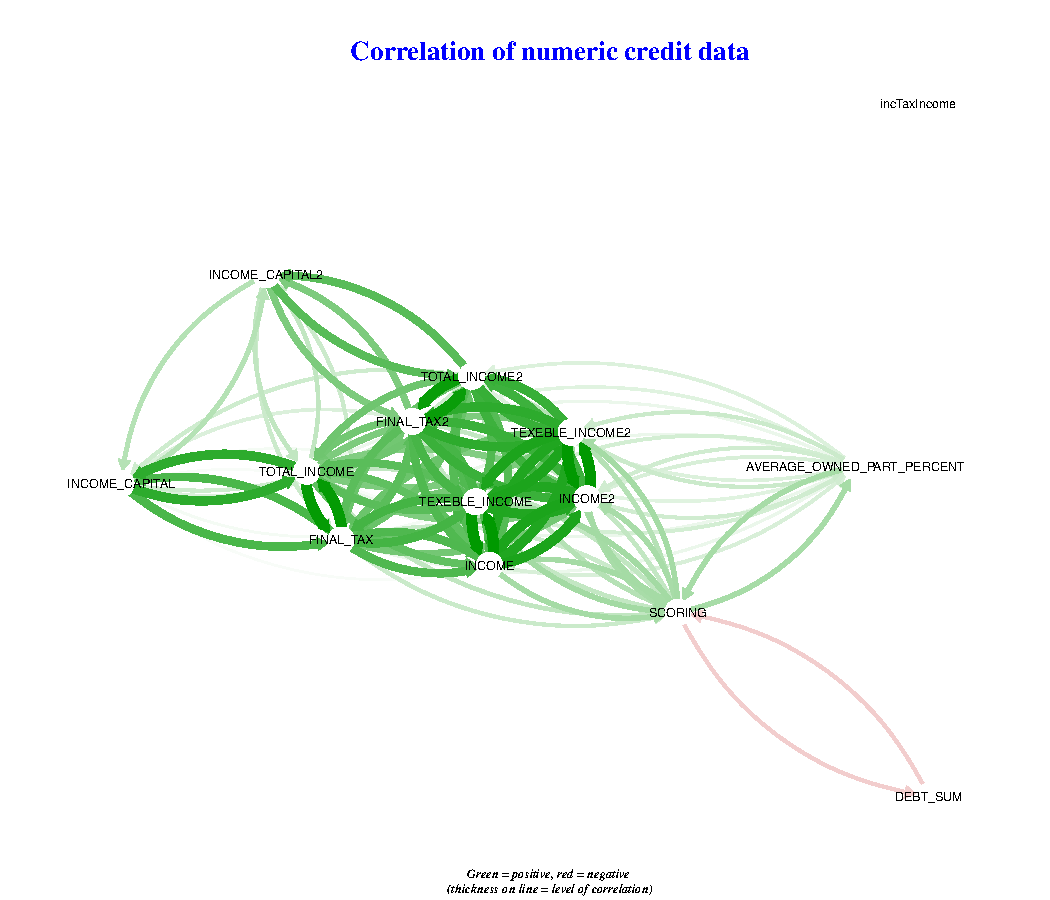
\includegraphics[width=0.65\textwidth,keepaspectratio]{CorrelationNumeric}
	}
}
\\
\subfloat[]{
\fbox{	
	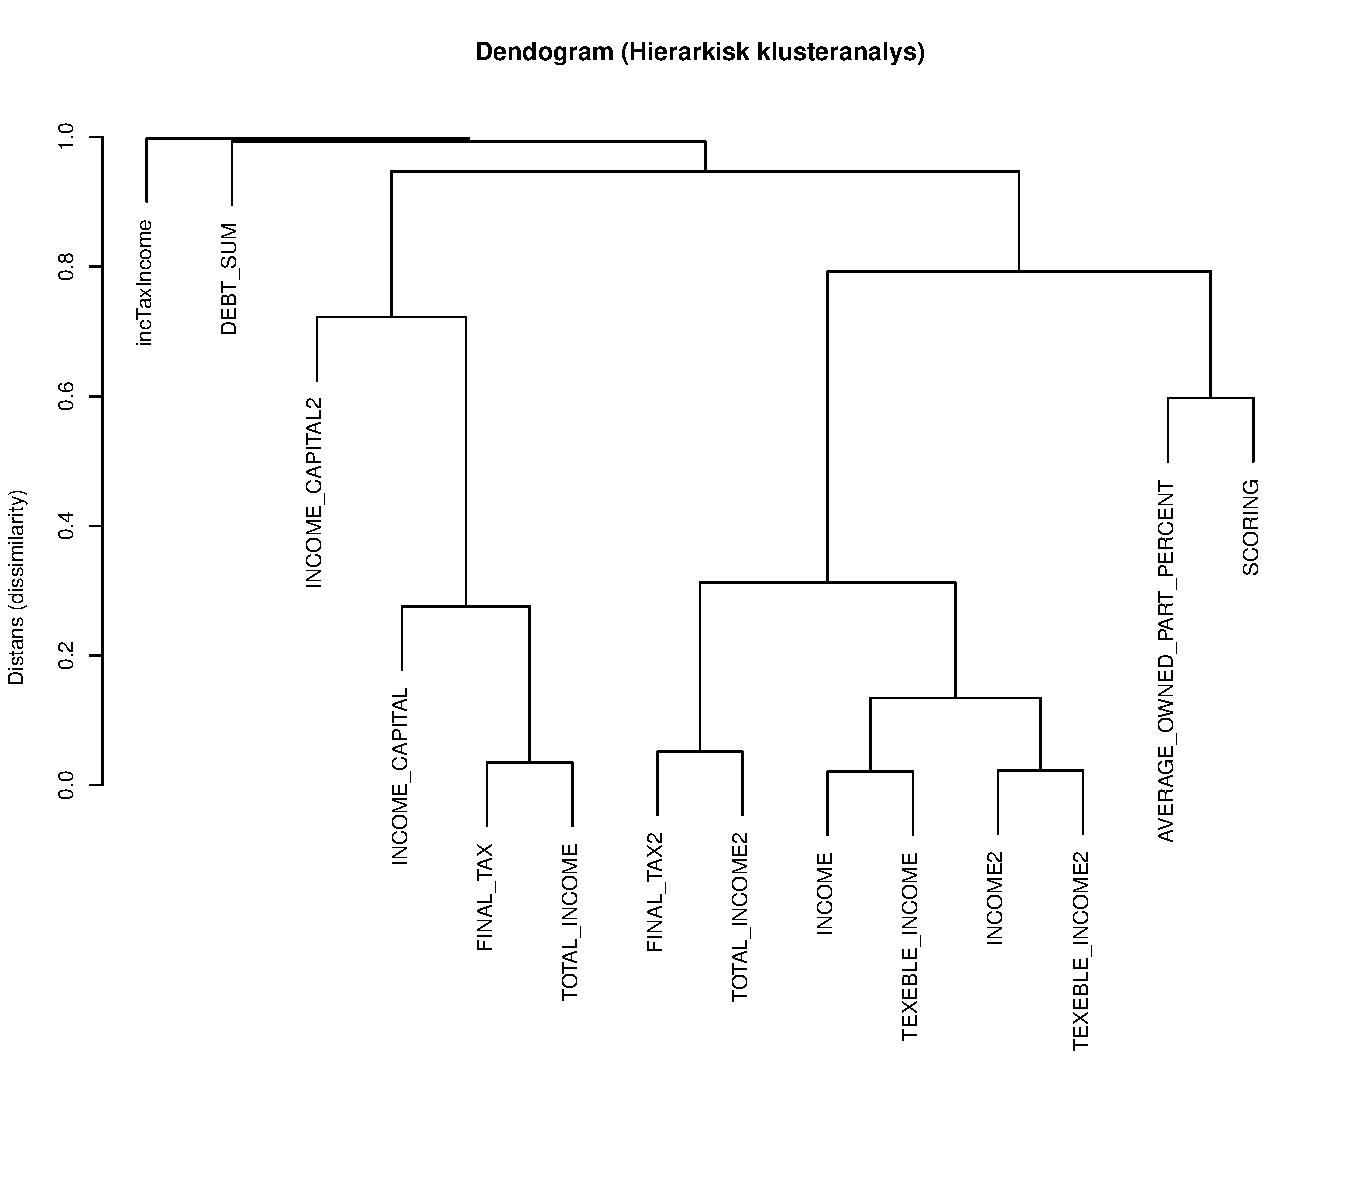
\includegraphics[width=0.65\textwidth,keepaspectratio]{Dendogram}
	}
}	
\label{fig:correlation}
\end{figure}
\clearpage


\section{Beslutsträd}

\begin{figure}[ht]
\centering
\caption{Caret och optimering}
\subfloat[]{
\fbox{	
	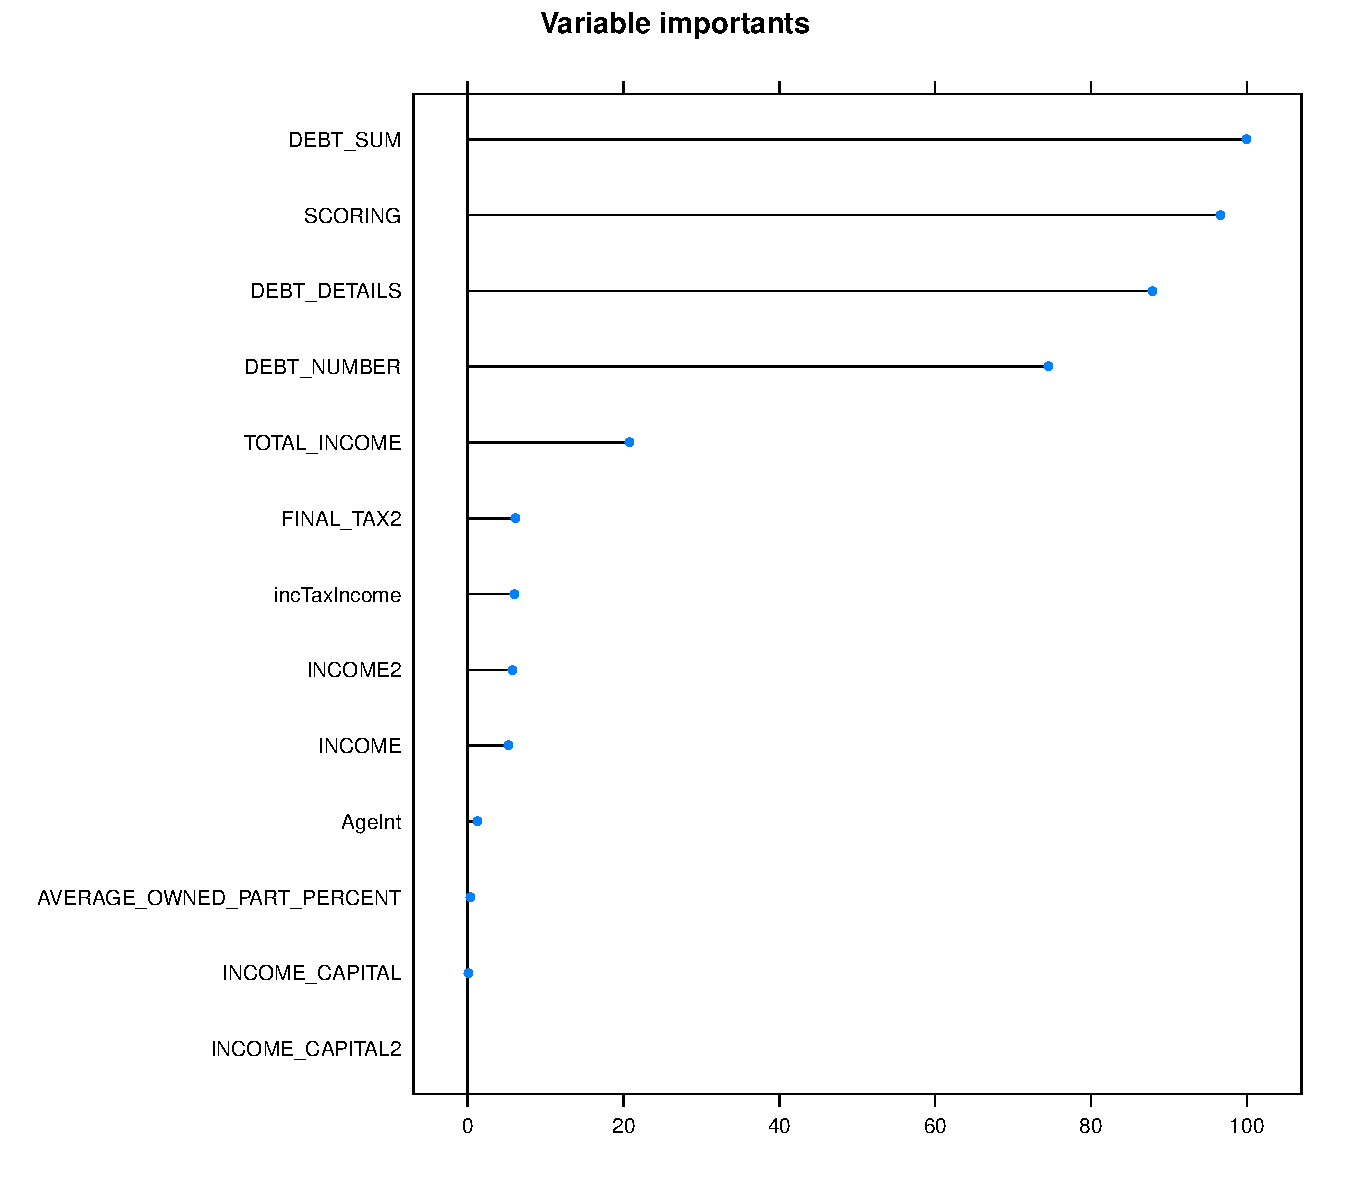
\includegraphics[width=0.65\textwidth,keepaspectratio]{VarImportants}
	}
}
\\
\subfloat[]{
\fbox{	
	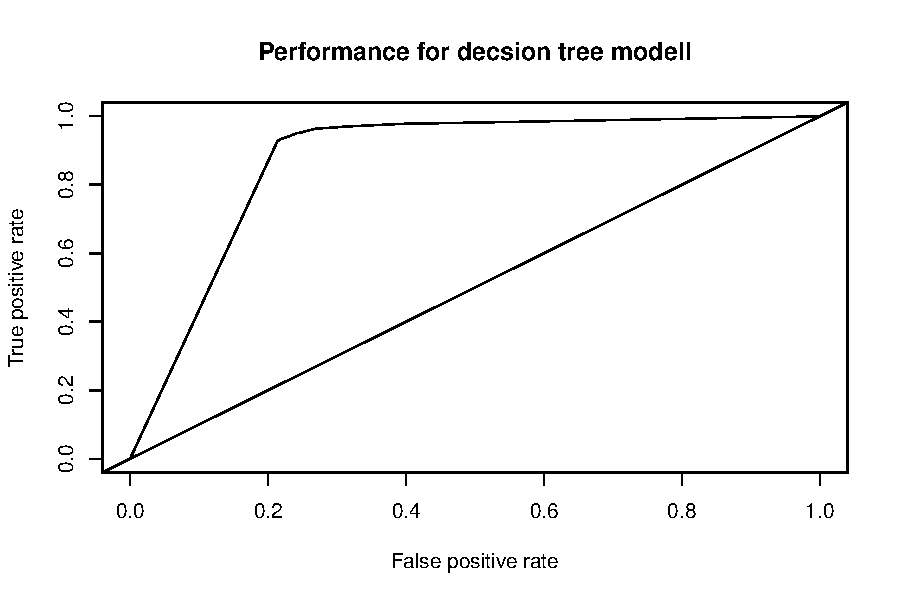
\includegraphics[width=0.65\textwidth,keepaspectratio]{ROCtree}
	}
}	
\label{fig:imp}
\end{figure}


\begin{landscape}
\thispagestyle{empty}
\begin{figure}
\caption{Beslutsträd, reducerat genom komplexitet parametern}
 \centering
  \makebox[0pt]{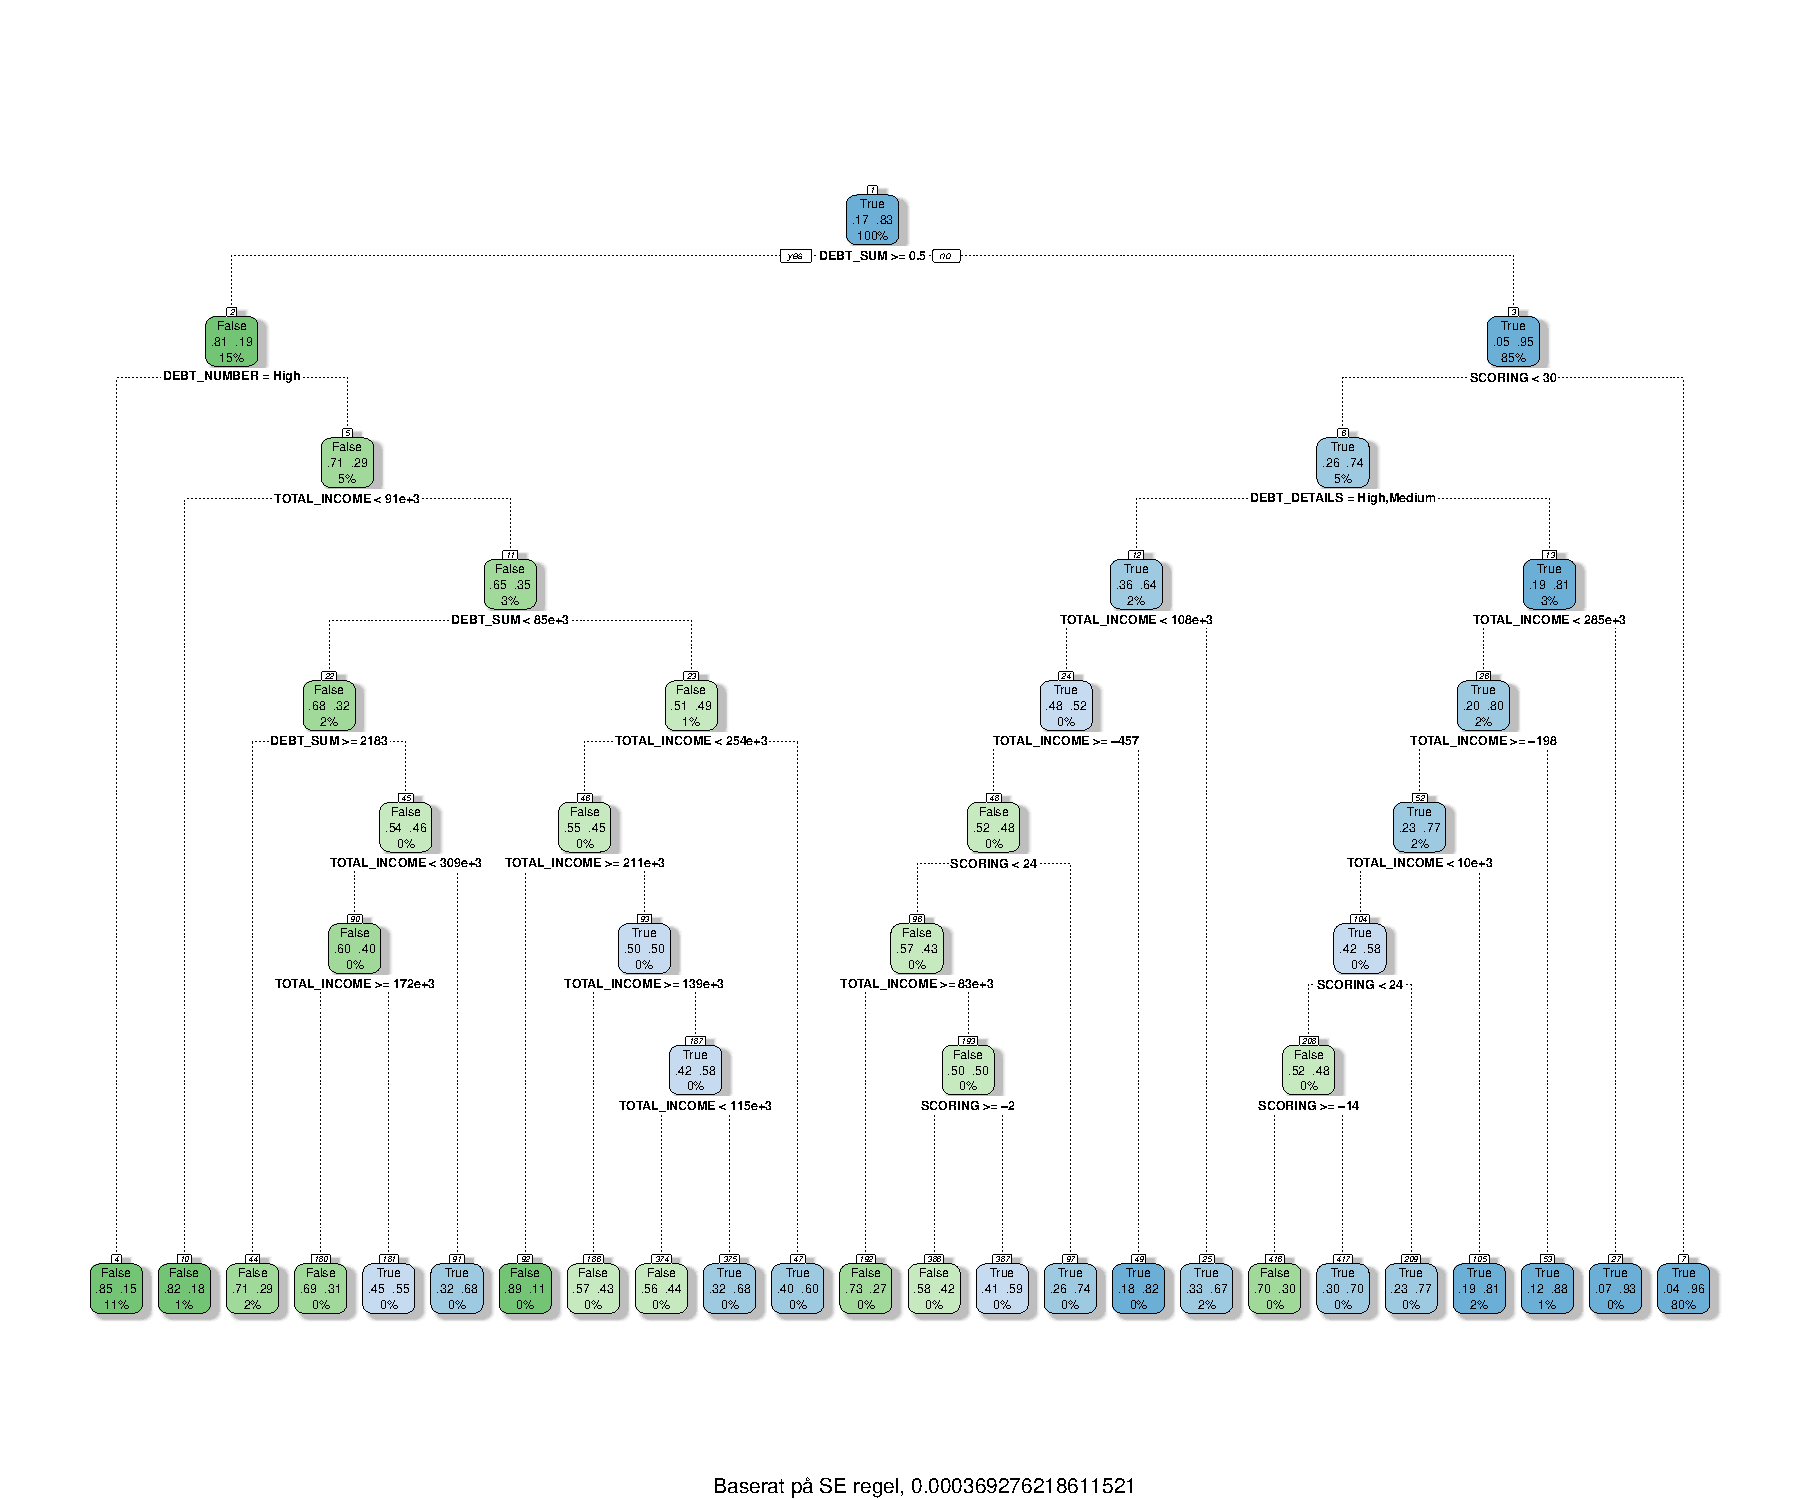
\includegraphics[width=20cm, keepaspectratio]{tree1}}
  \label{fig:tree1}
\end{figure}
\end{landscape}


\end{document}

